\chapter{Machinetaalmonitor}
\label{cha:MLMonitor}
\section{Inleiding}

Een machinetaalmonitor is een programma waarmee u de interne toestand van de processor en het geheugen van een computer kunt bekijken en ermee kunt experimenteren. Zo'n monitor is handig bij het opsporen van fouten in machinetaalprogramma's en bij het onderzoeken hoe de computer werkt. Een typische monitor kan onder meer de inhoud van de CPU-registers en van het geheugen weergeven en wijzigen, machinetaal disassembleren, instructies rechtstreeks in het geheugen assembleren en het geheugen op andere manieren bewerken.

De MEGA65 heeft twee afzonderlijke machinetaalmonitors ingebouwd: één in de ROM (de MEGA65-monitor) en één die deel uitmaakt van de Matrix Mode-debuginterface (de Matrix Mode/seriële monitor). Elke monitor heeft zijn eigen mogelijkheden en toepassingen.

De monitor in de ROM van de MEGA65 lijkt op de monitor die bij de oorspronkelijke C65-ROM hoorde, maar is vollediger en biedt meer mogelijkheden. Hij is opgenomen in zowel de gesloten MEGA65-ROM als in de uitgebreide MEGA65 OpenROM. Indien u een oorspronkelijke C65-ROM gebruikt, werkt de monitor daarin op vergelijkbare wijze.


\section{De machinetaalmonitor van de MEGA65}
\index{MONITOR!MEGA65-monitor}

De machinetaalmonitor die bij de ROM van de MEGA65 hoort, kunt u op verschillende manieren openen. Vanuit BASIC roept u de monitor aan met het commando {\screentext MONITOR}. U kunt er ook voor zorgen dat de MEGA65 rechtstreeks in de monitor opstart door tijdens het opstarten de toets \specialkey{STOP} ingedrukt te houden.

De MEGA65-monitor wordt automatisch geactiveerd wanneer het programma de instructie {\bf BRK} tegenkomt (bytewaarde {\tt 00}). U kunt uw programma op een specifiek punt laten pauzeren en de monitor openen, door op die plek in de programmacode een {\bf BRK}-instructie op te nemen.

Wanneer de monitor start, toont hij eerst de inhoud van de registers en wacht daarna op een commando:

\begin{tcolorbox}[colback=blue,coltext=white]
\verbatimfont{\codefont}
\begin{verbatim}
MONITOR
    PC   SR AC XR YR ZR BP SP
; 000000 00 00 00 00 00 00 F8
\end{verbatim}
\end{tcolorbox}

\subsection{Getallen}
\label{sec:numbers}

De monitor gebruikt hexadecimale notatie (grondtal 16) om getallen weer te geven, zoals geheugenadressen en waarden. Hexadecimale waarden verschijnen zonder voorafgaand `\$`-teken, zoals {\tt 5A} of {\tt D020}.

U kunt een waarde in hexadecimale, decimale (grondtal 10), octale (grondtal 8) of binaire (grondtal 2) notatie invoeren. Elk getalformaat gebruikt een teken als prefix, zoals in de onderstaande tabel staat. Indien u de prefix weglaat, gaat de monitor ervan uit dat de waarde hexadecimaal is. (Dat is anders dan bij BASIC, dat zonder prefix uitgaat van decimale notatie.) U kunt een bytewaarde ook als PETSCII-teken invoeren, met de bijbehorende prefix.

Ook voor instructies in assembleertaal is hexadecimaal het standaardgetalformaat. Dat kan verwarrend zijn! Bedenk wat er gebeurt als u de monitor de volgende instructie laat assembleren:

\begin{verbatim}
LDA #10
\end{verbatim}

Een gewone assembler ziet dit als het laden van de decimale waarde 10 (hex {\tt 0A}) in de accumulator. De monitor gaat er echter van uit dat dit de hexadecimale waarde {\tt \$10} is (decimaal 16). Om verwarring te voorkomen geeft u bij getallen in instructies in assembleertaal altijd expliciet een prefixteken op. De disassembler van de monitor toont alle waarden als hexadecimaal, beginnend met het prefix {\tt \$}.

Alle getallen moeten letterlijke waarden zijn. De monitor begrijpt geen rekenkundige uitdrukkingen.

U kunt de monitor ook gebruiken om een gegeven getal of PETSCII-teken in alle grondtallen te tonen. Typ daartoe het getal in alsof het een commando is, met de bijbehorende prefix. Voor hexadecimale getallen is de {\tt \$} in dit geval verplicht, om het onderscheid te maken met andere monitorcommando's.

In de volgende tabel staan de prefixes voor elke manier waarop u een waarde kunt invoeren:

{\ttfamily
{\setlength{\tabcolsep}{1mm}
\begin{center}
\begin{tabular}{|l|l|l|l|l|}
\hline
 grondtal  & naam & prefix & toegelaten tekens & voorbeeld     \\
\hline
16 & hexadecimaal &     & 0123456789ABCDEF &   100       \\16 & hexadecimaal & \$  & 0123456789ABCDEF & \$100       \\10 & decimaal     &  +  & 0123456789       & +256        \\ 8 & octaal       & \&  & 01234567         & \&400       \\ 2 & binair       & \%  & 01               & \%100000000 \\   & teken        &  '  & alle             & 'A          \\
\hline
\end{tabular}
\end{center}
}
}

\subsection{De assembler}

De monitor heeft een ingebouwde mini-assembler waarmee u machinetaal kunt schrijven met de standaardmnemonieken, zoals {\bf LDA} of {\bf STA}.

Dit is geen volwaardige assembler zoals u die zou gebruiken om grote programma's te schrijven. Met name ondersteunt hij geen symbolen, zoals labels voor subroutines of KERNAL-adressen. In plaats van {\ttfamily {\bf JSR CHROUT}} moet u het adres van {\ttfamily {\bf CHROUT}} opzoeken en de numerieke waarde ervan intypen: {\ttfamily {\bf JSR FFD2}}

Voor het gemak kunt u bij een vertakkingsinstructie een volledig adres opgeven. De monitor berekent dan de relatieve adresoffset om de instructie te assembleren.

De assembler kent alle instructies en adresseermethoden van de MEGA65-CPU 45GS02. Een instructie zoals {\ttfamily \bf LDA [TXTPTR],Z} wordt geassembleerd als het laden van de accumulator met behulp van een 32-bits pointer op de adressen {\ttfamily \bf TXTPTR, TXTPTR+1, TXTPTR+2, TXTPTR+3}.

\subsection{Verschillen met de C65-monitor}

De MEGA65-monitor lijkt op de monitor van de C65. Hij kent echter tal van uitbreidingen ten opzichte van de C65-monitor, zowel om de monitor in het algemeen nuttiger te maken als om hem uit te breiden met ondersteuning voor mogelijkheden die specifiek zijn voor de architectuur van de MEGA65.

De MEGA65-monitor beschikt over de volgende unieke mogelijkheden:

\begin{description}[leftmargin=1cm,style=nextline]
\item[Adressen:] Alle adressen worden gebruikt als 32-bits adressen (4 bytes). Zo krijgt u toegang tot het volledige adresbereik van de MEGA65, dat 28 bits beslaat. Dit is vooral nuttig voor de toegang tot de RAM-blokken van 8 MB: attic RAM op \$8000000 (ingebouwd) en cellar RAM op \$8800000 (optioneel). Stelt u bit 31 van een adres in op 1, dan krijgt u toegang tot een speciale (in banken ingedeelde) configuratie. In dat geval bedekken het I/O-gebied op \$D000 en de ROM-gebieden \$6000 - \$7FFF (monitor-ROM) en \$E000 - \$FFFF (KERNAL-ROM) de huidige bank.

\item[Commando's:] Het extra commando {\bf B} geeft bitmaps van tekens weer.

\item[Schijftoegang:] Het schijfcommandoteken {\bf \@} kent twee extra functies: {\bf U1} om een reeks schijfblokken naar het geheugen te lezen en {\bf U2} om een geheugenbereik naar schijfblokken te schrijven. Dit maakt het bewerken van schijven mogelijk, bijvoorbeeld het wijzigen van directory-items, maar u kunt het zelfs gebruiken om een back-up te maken van de volledige inhoud van diskettes of schijfimages. De attic RAM is groot genoeg om de inhoud van 8 volledige 1581-diskettes te bevatten.

\item[Disassembler:] De disassembler kan alle extra adresseermethoden decoderen, zoals de 32-bits indirecte modus $[\$nn],Z$ en de samengestelde instructies die het 32-bits Q-register gebruiken.

\item[Register:] Het registeroverzicht toont de volledige 16-bits stackpointer en het Base-Page-register en aanvaardt nieuwe instellingen voor beide.

\end{description}



\subsection{Tabel met MEGA65-monitorcommando's}

{
\ttfamily
\setlength{\tabcolsep}{1mm}
\begin{center}
\begin{tabular}{|l|l|L{6.5cm}|}
\hline
C & mnemoniek & beschrijving \\
\hline
A &     ASSEMBLE        & Assembleert een regel 45GS02-code\\B &     BITMAPS         & Geeft 8x8-bitmaps (tekens) weer\\C &     COMPARE         & Vergelijkt twee geheugengebieden\\D &     DISASSEMBLE     & Disassembleert een regel 45GS02-code\\F &     FILL            & Vult een geheugengebied met een waarde \\G &     GO              & Start de uitvoering op het opgegeven adres\\H &     HUNT            & Zoekt opgegeven gegevens in een geheugengebied\\J &     JUMP            & Springt naar een subroutine op het opgegeven adres\\L &     LOAD            & Laadt een bestand van schijf\\M &     MEMORY          & Toont een geheugengebied\\R &     REGISTERS       & Toont de inhoud van de 45GS02-registers\\S &     SAVE            & Slaat een geheugengebied op in een schijfbestand\\T &     TRANSFER        & Kopieert geheugen naar een andere locatie\\V &     VERIFY          & Vergelijkt een geheugengebied met een schijfbestand\\X &     EXIT            & Verlaat de monitormodus\\
\hline
 . &     <punt>          & Assembleert een regel 45GS02-code\\ > &     <groter dan>    & Wijzigt het geheugen\\ ; &     <puntkomma>     & Wijzigt de registerinhoud\\ @ &     <apestaartje>      & Schijfcommando, directory of status\\
\hline
\$ &     <hex>           & Geeft de waarde in hexadecimaal, decimaal, octaal en binair weer \\ + &     <decimaal>      & Geeft de waarde in hexadecimaal, decimaal, octaal en binair weer\\\& &     <octaal>        & Geeft de waarde in hexadecimaal, decimaal, octaal en binair weer\\\% &     <binair>        & Geeft de waarde in hexadecimaal, decimaal, octaal en binair weer\\
\hline
\end{tabular}
\end{center}
}

% ======================================
% Start of the monitor command reference
% ======================================

\titleformat*{\subsubsection}{\normalfont\huge\bfseries\color{blue}}

% ********
% ASSEMBLE
% ********

\subsubsection{A : ASSEMBLE}

\index{ASSEMBLE}
\index{MONITOR-commando's!ASSEMBLE}
\begin{description}[leftmargin=2cm,style=nextline]
\item [Formaat:] {\bf A adres mnemoniek operand}\item [Gebruik:] Met de mini-assembler voert u machinetaalinstructies in met behulp van gemakkelijk te onthouden mnemonieken in plaats van opcodes. De operand kunt u invoeren als hexadecimaal getal, decimaal getal, binair getal of teken. Sprongdoelen worden automatisch omgerekend naar relatieve afstanden. Na elke ingevoerde instructie genereert de mini-assembler de 1 tot 5 bytes lange machinetaal, drukt deze code samen met de instructie af en verhoogt de programmateller. Er verschijnt een nieuwe regel met het commando {\bf A}, waarin de nieuwe waarde van de programmateller wordt afgedrukt. Dit vergemakkelijkt het snel invoeren van instructies. De assembleerinvoermodus wordt uitsluitend beëindigd door op RETURN te drukken. U kunt elke regel van de ingevoerde code of een regel in disassembly-indeling wijzigen door de cursor naar die regel te verplaatsen en het gewenste element te veranderen, bijvoorbeeld de mnemoniek of de operand. Hexadecimale waarden die vóór de mnemoniek staan, worden genegeerd.

Indien u na het uitvoeren van de code wilt terugkeren naar de monitor, moet de laatste instructie een {\bf BRK}-instructie zijn en moet het programma worden aangeroepen terwijl I/O en de monitor-ROM actief zijn. Dat doet u door bit 31 van het uitvoeradres in te stellen. Indien het programma in bank 0 op adres 1500 is ingevoerd, start u het met: \screentext{G 80001500}.

Indien de ingevoerde code een subroutine is, moet deze eindigen met een {\bf RTS}-instructie.

\item [Opmerkingen:] De assembler herkent alle 45GS02-instructies van de MEGA65, met inbegrip van de instructies die het Q-register gebruiken. {\bf NOP} en {\bf AUG} kunnen worden ingevoerd, maar worden geïnterpreteerd als {\bf EOM} respectievelijk {\bf MAP}.

32-bits Base-Page-Indirect-instructies gebruiken vierkante haken ({\bf [} en {\bf ]}).

\end{description}
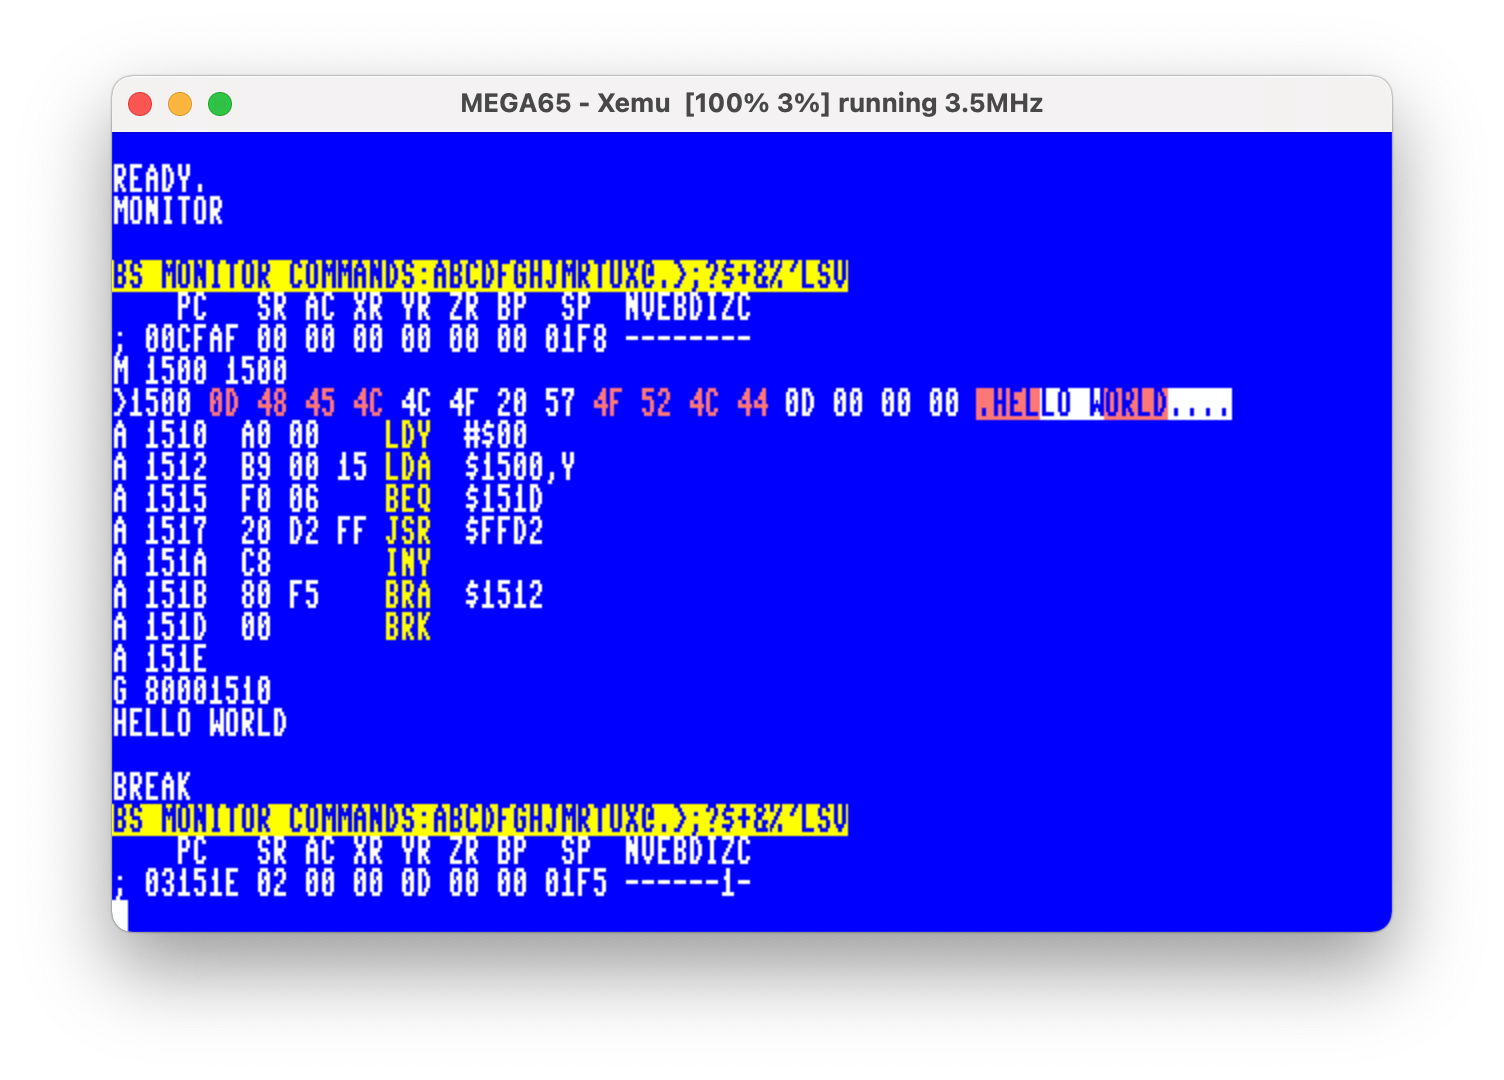
\includegraphics[width=\linewidth]{images/monitor-a}

% *******
% BITMAPS
% *******

\subsubsection{B : BITMAPS}

\index{BITMAPS}
\index{MONITOR-commando's!BITMAPS}
\begin{description}[leftmargin=2cm,style=nextline]
\item [Formaat:] {\bf B begin}\item [Gebruik:] Geeft geheugenwaarden weer, geïnterpreteerd als bitmaps van tekens.

\item [Opmerkingen:] Het commando B geeft de inhoud van geheugencellen bitsgewijs weer, waarbij voor een 1 een sterretje en voor een 0 een punt wordt afgedrukt. Daarbij wordt rekening gehouden met de bijzondere indeling van tekengegevens, waarbij 8 bytes samen één tekencel vormen. Bij elke aanroep worden 8 tekens weergegeven.

In de {\tt 92XXXX}-ROM's zijn drie ROM-tekensets ingebouwd:

\begin{tcolorbox}[colback=blue,coltext=white]
\verbatimfont{\codefont}
\begin{verbatim}
FONT A : REM $029000 : ASCII [\]^_ {|}~ inbegrepen
FONT B : REM $03D000 : versie van A met schreef
FONT C : REM $02D000 : origineel C64-lettertype
\end{verbatim}
\end{tcolorbox}
\end{description}
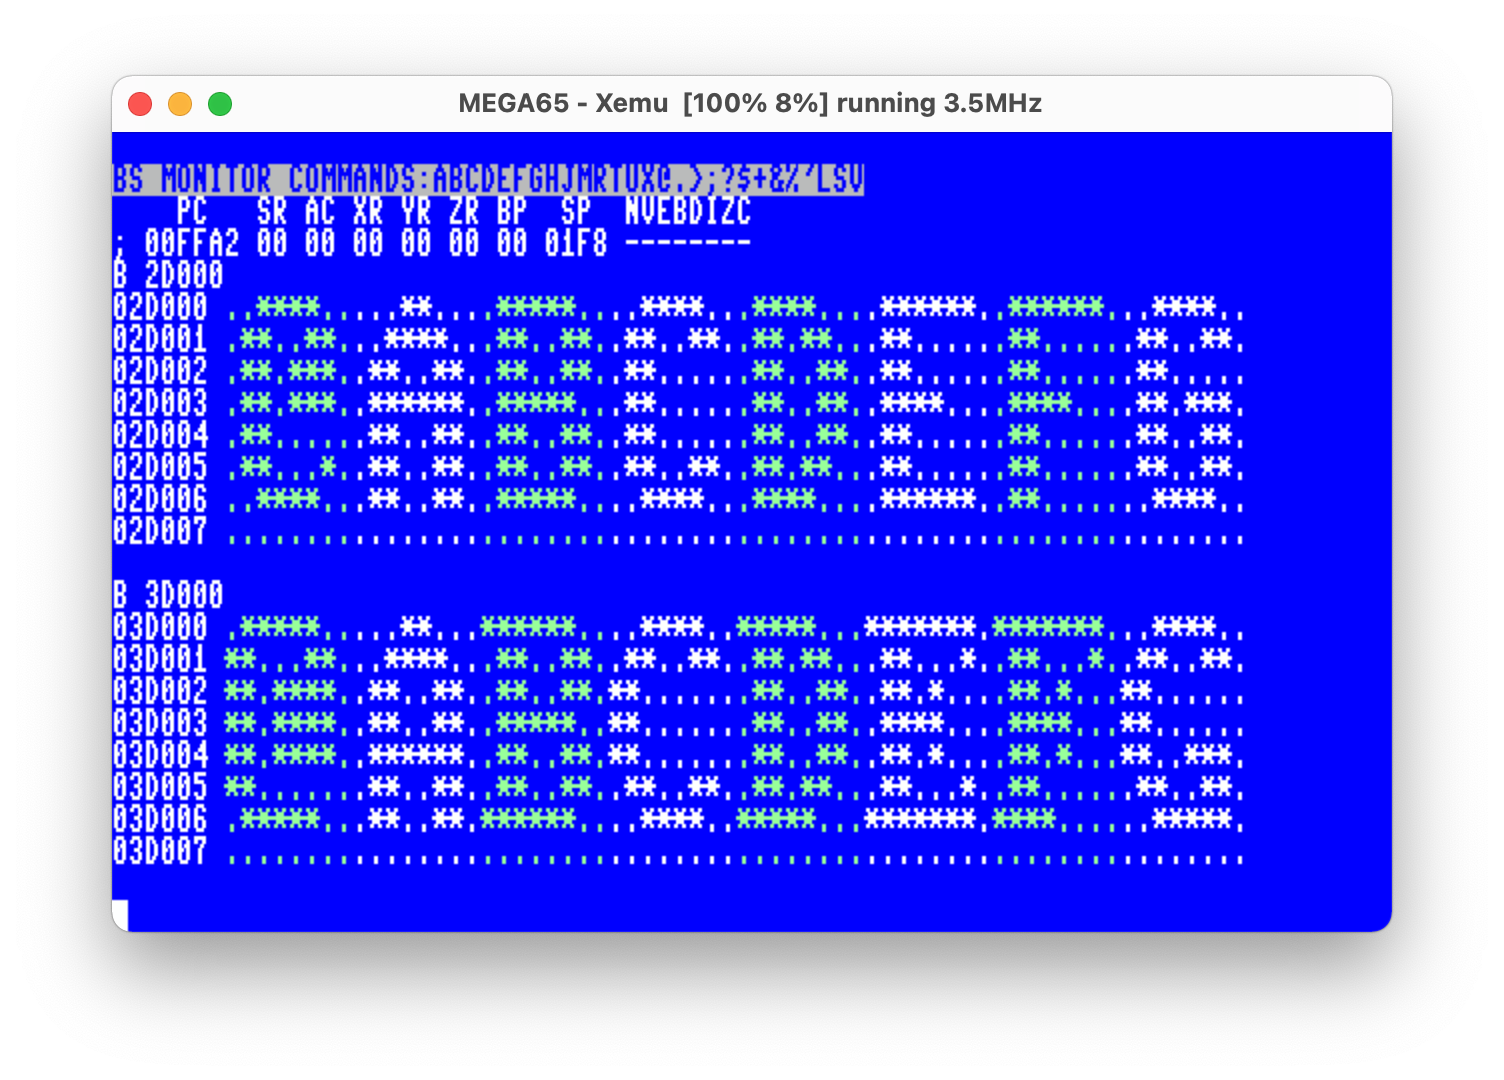
\includegraphics[width=\linewidth]{images/monitor-b}

% *******
% COMPARE
% *******

\subsubsection{C : COMPARE}
\index{COMPARE}
\index{MONITOR-commando's!COMPARE}
\begin{description}[leftmargin=2cm,style=nextline]
\item [Formaat:] {\bf C begin einde begin-b}\item [Gebruik:] Vergelijkt twee geheugengebieden en geeft vervolgens de adressen weer waarvan de waarden verschillen.

\item [Opmerkingen:] Het eindadres ligt één adres voorbij het laatste te vergelijken adres.

    Het tweede geheugengebied dat vergeleken wordt, begint op {\bf begin-b} en heeft dezelfde grootte als het gebied dat door {\bf begin} en {\bf einde} wordt omschreven.

    Adressen worden als hexadecimale waarden weergegeven.

\end{description}
% TODO: screenshot  \includegraphics[width=\linewidth]{images/monitor-c}

% ***********
% DISASSEMBLE
% ***********

\subsubsection{D : DISASSEMBLE}
\index{DISASSEMBLE}
\index{MONITOR-commando's!DISASSEMBLE}
\begin{description}[leftmargin=2cm,style=nextline]
\item [Formaat:] {\bf D [van [tot]]}\item [Gebruik:] Toont een listing in machinetaal voor het opgegeven adresbereik, in de veronderstelling dat het code bevat. Wanneer slechts één argument is opgegeven, disassembleert de disassembler de volgende 21 bytes. Indien geen argument is opgegeven, gaat de disassembly verder op het laatst gebruikte adres voor disassemblage. De inhoud wordt als hexadecimale waarden weergegeven.

\item [Opmerkingen:] De regels beginnen met het puntteken '.'. Hierdoor kunt u de disassembly direct op het volledige scherm bewerken. Drukt u in een willekeurige regel RETURN in, dan assembleert de monitor het gewijzigde commando van de cursorregel weer naar het geheugen, indien zich daar schrijfbare RAM bevindt. Zie het monitorcommando {\bf .}.

                 De disassembler kent de instructieset van de MEGA65-CPU, de
                 45GS02. Heeft een instructie het voorvoegsel {\bf NEG NEG}, dan worden
                 die hexadecimale waarden weggelaten en verschijnt in plaats daarvan
                 een sterretje ({\bf *}) tussen het adres en de hexadecimale waarden.

\item [Voorbeeld:] Gebruik van {\bf D}
\end{description}
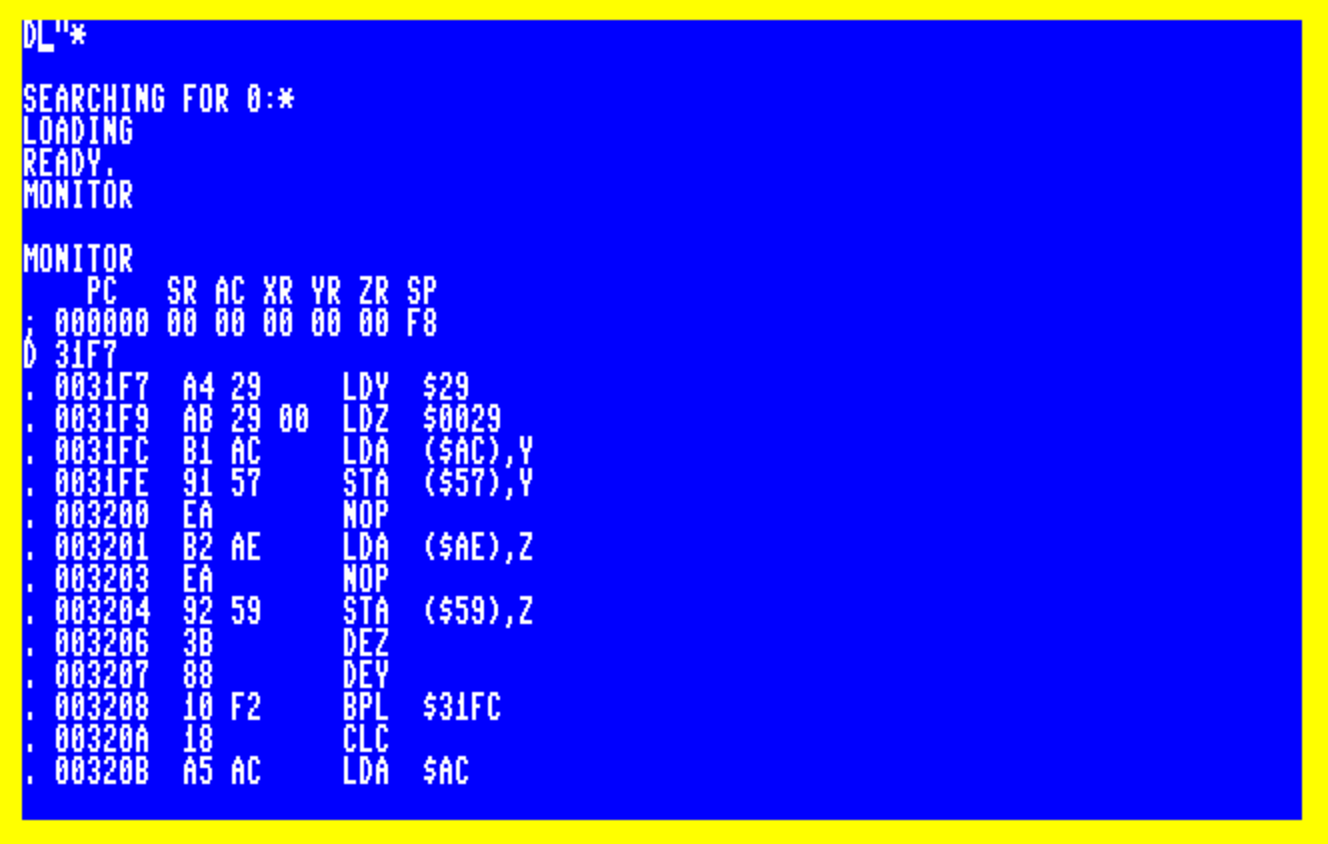
\includegraphics[width=\linewidth]{images/monitor-d}

% ****
% FILL
% ****

\subsubsection{F : FILL}
\index{FILL}
\index{MONITOR-commando's!FILL}
\begin{description}[leftmargin=2cm,style=nextline]
\item [Formaat:] {\bf F begin einde waarde}\item [Gebruik:] Vult een geheugengebied met een waarde.

\item [Opmerkingen:] Het eindadres ligt één adres voorbij het laatste adres dat gevuld wordt.
\end{description}
% TODO: screenshot  \includegraphics[width=\linewidth]{images/monitor-f}

% **
% GO
% **

\subsubsection{G : GO}
\index{GO}
\index{MONITOR-commando's!GO}
\begin{description}[leftmargin=2cm,style=nextline]
\item [Formaat:] {\bf G [adres]}\item [Gebruik:] Voert de code op een adres uit. Wordt {\bf adres} weggelaten, dan gebruikt de monitor de huidige programmateller als adres.

\item [Opmerkingen:] Dit is gelijkwaardig aan een {\bf JMP}-instructie.

    Het commando {\bf G} zonder argument is een handige manier om de uitvoering van een programma te hervatten nadat de monitor met een {\bf BRK}-instructie is gestart.

    Omdat dit een {\bf JMP} gebruikt, mag u dit commando niet gebruiken om subroutines aan te roepen. Zie {\bf J}.

\end{description}
% TODO: screenshot  \includegraphics[width=\linewidth]{images/monitor-g}

% ****
% HUNT
% ****

\subsubsection{H : HUNT}
\index{HUNT}
\index{MONITOR-commando's!HUNT}
\begin{description}[leftmargin=2cm,style=nextline]
\item [Formaat:] {\bf H begin einde byte [byte...]}\item [Gebruik:] Zoekt in een bereik van het geheugen naar elk voorkomen van een bytereeks en geeft vervolgens het beginadres van elk voorkomen weer.

\item [Opmerkingen:] Het eindadres ligt één adres voorbij het laatste adres dat doorzocht wordt.

    Adressen worden als hexadecimale waarden weergegeven.

\end{description}
% TODO: screenshot  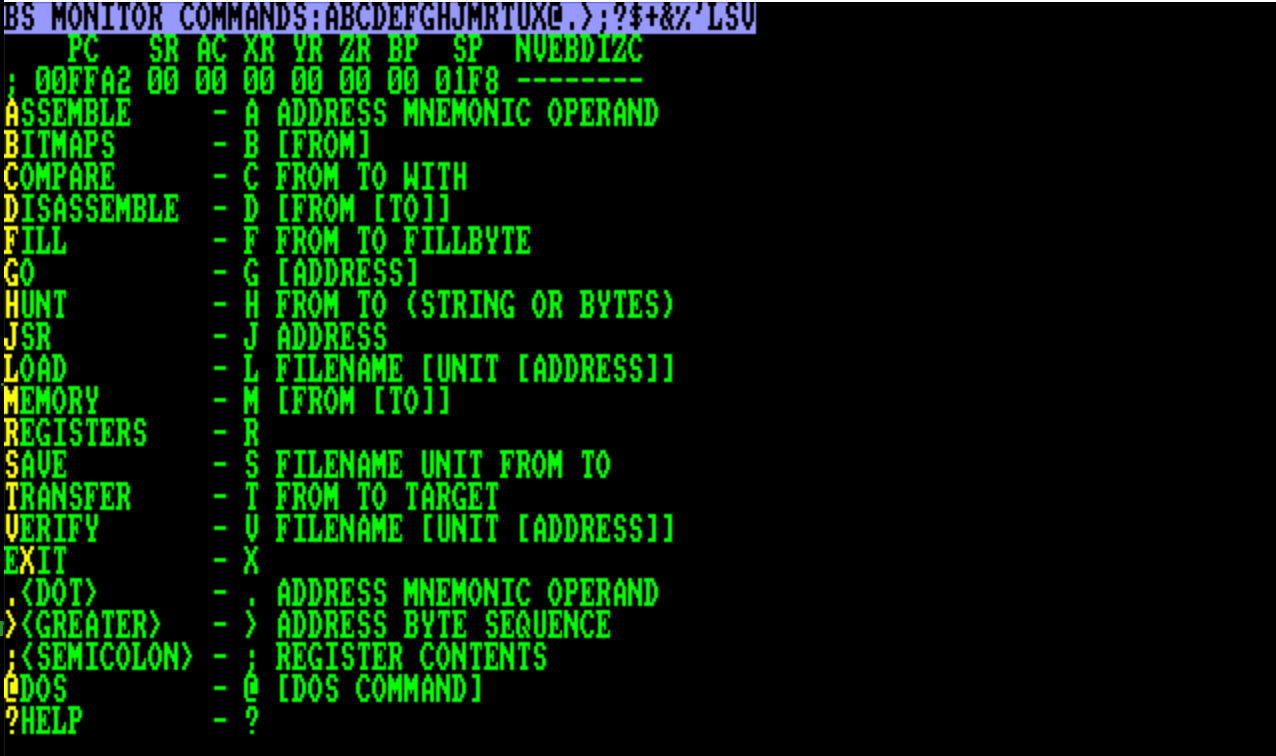
\includegraphics[width=\linewidth]{images/monitor-h}

% ****
% JUMP
% ****

\subsubsection{J : JUMP}
\index{JUMP}
\index{MONITOR-commando's!JUMP}
\begin{description}[leftmargin=2cm,style=nextline]
\item [Formaat:] {\bf J adres}\item [Gebruik:] Springt naar een subroutine op een adres.

\item [Opmerkingen:] Dit is gelijkwaardig aan een {\bf JSR}-instructie. Keert de subroutine terug met {\tt RTS}, dan neemt de monitor het weer over.

    Wilt u de uitvoering gewoon op een adres voortzetten zonder terugkeer naar de monitor te verwachten, gebruik dan {\bf G}.

\end{description}
% TODO: screenshot  \includegraphics[width=\linewidth]{images/monitor-j}

% ****
% LOAD
% ****

\subsubsection{L : LOAD}
\index{LOAD}
\index{MONITOR-commando's!LOAD}
\begin{description}[leftmargin=2cm,style=nextline]
\item [Formaat:] {\bf L "bestandsnaam",eenheid [begin]}\item [Gebruik:] Laadt gegevens uit een bestand in het geheugen.

\item [Opmerkingen:] De bestandsnaam moet tussen dubbele aanhalingstekens staan.

    Het nummer van de {\bf eenheid} (zoals 8 of 9) is verplicht. {\bf Eenheid} wordt opgegeven in het normale talstelsel van de monitor (standaard hexadecimaal). Zie \hyperref[sec:numbers]{Getallen}.

    Ontbreekt het {\bf begin}-adres, dan neemt de monitor het beginadres uit de eerste twee bytes van het bestand. Het bestand moet van het type {\tt PRG} zijn. Indien u {\bf begin} opgeeft, negeert de monitor de {\tt PRG}-kop van twee bytes.

\end{description}
% TODO: screenshot  \includegraphics[width=\linewidth]{images/monitor-l}

% ******
% MEMORY
% ******

\subsubsection{M : MEMORY}
\index{MEMORY}
\index{MONITOR-commando's!MEMORY}
\begin{description}[leftmargin=2cm,style=nextline]
\item [Formaat:] {\bf M [van [,tot]]}\item [Gebruik:] Drukt een geheugendump af voor het opgegeven adresbereik. De dump toont de geheugeninhoud, ingedeeld in rijen van 16 opeenvolgende adressen, te beginnen met het adres dat als eerste argument is opgegeven. De dump loopt door totdat een rij is afgedrukt die de waarde bevat van het adres dat als tweede argument is opgegeven. Ontbreekt het tweede argument, dan toont de dump een volledige pagina van 256 bytes in 16 rijen. De inhoud wordt afgedrukt als 16 bytewaarden in hexadecimale notatie, gevolgd door de tekenweergave.

\item [Opmerkingen:] De rijen beginnen met het teken '>'. Hierdoor kunt u de dump direct op het volledige scherm bewerken. Drukt u in een willekeurige rij RETURN in, dan schrijft de monitor de gewijzigde waarden van de cursorrij terug naar het geheugen, indien zich daar schrijfbare RAM bevindt. Zie het monitorcommando {\bf >}.

\item [Voorbeeld:] Gebruik van {\bf M}
\end{description}
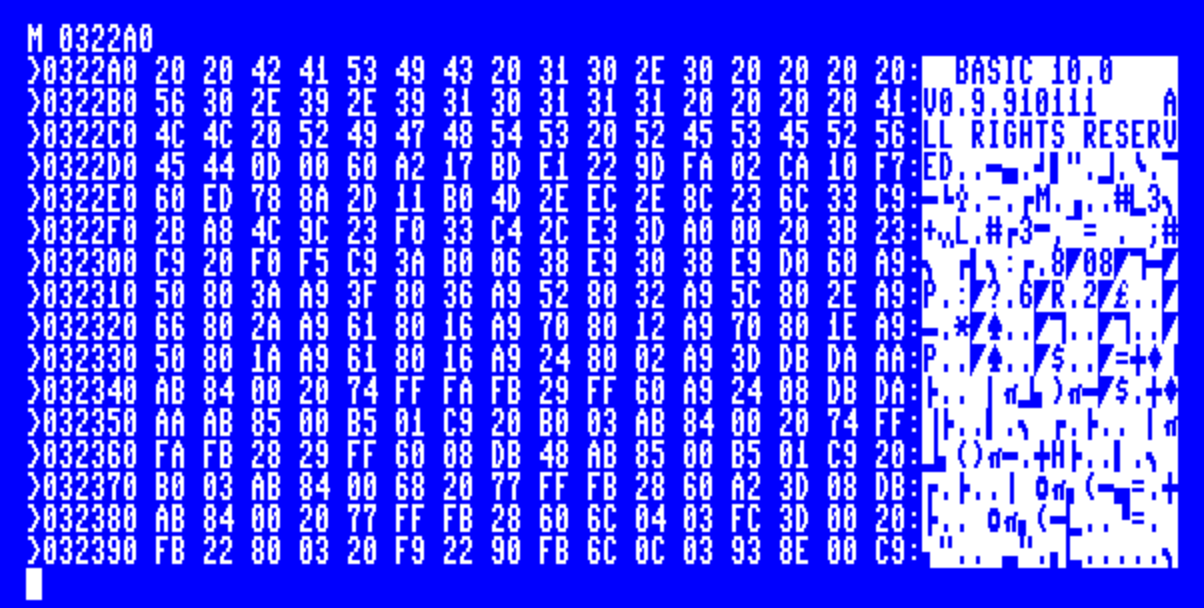
\includegraphics[width=\linewidth]{images/monitor-m}

% *********
% REGISTERS
% *********

\subsubsection{R : REGISTERS}
\index{REGISTERS}
\index{MONITOR-commando's!REGISTERS}
\begin{description}[leftmargin=2cm,style=nextline]
\item [Formaat:] {\bf R}\item [Gebruik:] Toont de inhoud van de registers zoals die waren vlak voordat de monitor werd gestart.

\item [Opmerkingen:] De uitvoer begint met het teken {\tt ;}, zodat u de registerwaarden kunt wijzigen door de cursor omhoog naar de regel te bewegen, de waarden aan te passen en vervolgens op \specialkey{RETURN} te drukken.

\end{description}
% TODO: screenshot  \includegraphics[width=\linewidth]{images/monitor-r}

% ****
% SAVE
% ****

\subsubsection{S : SAVE}
\index{SAVE}
\index{MONITOR-commando's!SAVE}
\begin{description}[leftmargin=2cm,style=nextline]
\item [Formaat:] {\bf S "bestandsnaam",eenheid begin einde}\item [Gebruik:] Slaat een geheugengebied op in een bestand op schijf, van het type {\tt PRG}.

\item [Opmerkingen:] De bestandsnaam moet tussen dubbele aanhalingstekens staan.

    Het nummer van de {\bf eenheid} (zoals 8 of 9) is verplicht. {\bf Eenheid} wordt opgegeven in het normale talstelsel van de monitor (standaard hexadecimaal). Zie \hyperref[sec:numbers]{Getallen}.

    Het eindadres ligt één adres voorbij het laatste adres dat opgeslagen wordt.

    Om een bestaand bestand te overschrijven, plaatst u {\tt 0:} vóór de bestandsnaam, bijvoorbeeld: {\tt "0:MYFILE"}.

\end{description}
% TODO: screenshot  \includegraphics[width=\linewidth]{images/monitor-s}

% ********
% TRANSFER
% ********

\subsubsection{T : TRANSFER}
\index{TRANSFER}
\index{MONITOR-commando's!TRANSFER}
\begin{description}[leftmargin=2cm,style=nextline]
\item [Formaat:] {\bf T begin einde bestemmingsbegin}\item [Gebruik:] Kopieert een geheugengebied naar een ander gebied.

\item [Opmerkingen:] Het eindadres ligt één adres voorbij het laatste adres dat gekopieerd wordt.

    De monitor veronderstelt dat het doelgebied even lang is als het brongebied. Alle bytes worden gekopieerd.

\end{description}
% TODO: screenshot  \includegraphics[width=\linewidth]{images/monitor-t}

% ******
% VERIFY
% ******

\subsubsection{V : VERIFY}
\index{VERIFY}
\index{MONITOR-commando's!VERIFY}
\begin{description}[leftmargin=2cm,style=nextline]
\item [Formaat:] {\bf V "bestandsnaam",eenheid begin}\item [Gebruik:] Controleert of een geheugengebied overeenkomt met een bestand op schijf.

\item [Opmerkingen:] De bestandsnaam moet tussen dubbele aanhalingstekens staan.

    Het nummer van de {\bf eenheid} (zoals 8 of 9) is verplicht. {\bf Eenheid} wordt opgegeven in het normale talstelsel van de monitor (standaard hexadecimaal). Zie \hyperref[sec:numbers]{Getallen}.

    De monitor veronderstelt dat de te controleren gegevens even lang zijn als het bestand.

    Komen de gegevens in het geheugen niet overeen, dan toont de monitor een foutmelding. Anders verschijnt er niets meer en kunt u ervan uitgaan dat de controle is geslaagd.

\end{description}
% TODO: screenshot  \includegraphics[width=\linewidth]{images/monitor-v}

% ****
% EXIT
% ****

\subsubsection{X : EXIT}
\index{EXIT}
\index{MONITOR-commando's!EXIT}
\begin{description}[leftmargin=2cm,style=nextline]
\item [Formaat:] {\bf X}\item [Gebruik:] Verlaat de monitor en keert terug naar BASIC.

\item [Opmerkingen:] Indien de monitor werd gestart door een {\bf BRK}-instructie in een programma, betekent het verlaten van de monitor in feite dat het programma wordt afgebroken. Om een gepauzeerd programma voort te zetten, gebruikt u in plaats daarvan {\bf G}.

\end{description}

% ************
% . (ASSEMBLE)
% ************

\subsubsection{. : ASSEMBLE}
\index{MONITOR-commando's!.}
\begin{description}[leftmargin=2cm,style=nextline]
\item [Formaat:] {\bf . adres opcode operand}\item [Gebruik:] Een alias voor {\bf A}.

\item [Opmerkingen:] De uitvoer van de disassembler begint elke regel met het teken {\tt .}. U kunt de door de disassembler afgedrukte machinetaalinstructies bewerken door de cursor omhoog naar een regel te bewegen, de regel aan te passen en vervolgens op \specialkey{RETURN} te drukken. Hierdoor verandert het {\tt .} in een {\tt A}, zodat u kunt zien welke regels opnieuw zijn geassembleerd.

\end{description}
% TODO: screenshot  \includegraphics[width=\linewidth]{images/monitor-dot}

% *****************
% > (MODIFY MEMORY)
% *****************

\subsubsection{> : MODIFY MEMORY}
\index{MONITOR-commando's!>}
\begin{description}[leftmargin=2cm,style=nextline]
\item [Formaat:] {\bf > adres byte [byte...]}\item [Gebruik:] Wijzigt één of meer bytes vanaf een adres.

\item [Opmerkingen:] De uitvoer van het commando {\bf M} begint elke regel met het teken {\tt >}. U kunt de door het commando {\bf M} afgedrukte geheugenwaarden bewerken door de cursor omhoog naar een regel te bewegen, de regel aan te passen en vervolgens op \specialkey{RETURN} te drukken.

\end{description}
% TODO: screenshot  \includegraphics[width=\linewidth]{images/monitor-gt}

% ********************
% ; (MODIFY REGISTERS)
% ********************

\subsubsection{; : MODIFY REGISTERS}
\index{MONITOR-commando's!.}
\begin{description}[leftmargin=2cm,style=nextline]
\item [Formaat:] {\bf ; pc sr ac xr yr zr bp sp nvebdizc}\item [Gebruik:] Wijzigt de CPU-registers. De argumenten hebben dezelfde indeling als de uitvoer van het commando {\bf R}.

\item [Opmerkingen:] De uitvoer van het commando {\bf R} begint de regel met het teken {\tt ;}. U kunt de door het commando {\bf R} afgedrukte registerwaarden bewerken door de cursor omhoog naar de regel te bewegen, de regel aan te passen en vervolgens op \specialkey{RETURN} te drukken.

\end{description}
% TODO: screenshot  \includegraphics[width=\linewidth]{images/monitor-semi}

% ****************
% @ (DISK COMMAND)
% ****************

\subsubsection{@ : DISK COMMAND}
\index{MONITOR-commando's!@}
\begin{description}[leftmargin=2cm,style=nextline]
\item [Formaat:] {\bf @ [eenheid] [,commando]}\item [Gebruik:] Voert een schijfcommando uit.

\item [Opmerkingen:] Zonder {\bf commando} toont dit de status van het schijfstation.

    Standaard is de {\bf eenheid} 8. De {\bf eenheid} wordt opgegeven in het normale talstelsel van de monitor (standaard hexadecimaal). Zie \hyperref[sec:numbers]{Getallen}.

    Een {\bf commando} van {\bf \$[pattern]} vraagt bij de opgegeven {\bf eenheid} een directoryoverzicht op en toont dit. U kunt optioneel een {\bf patroon} opgeven om de getoonde bestanden te beperken. De jokertekens {\bf *} en {\bf ?} kunnen worden gebruikt

    Het {\bf commando} kan elk Commodore-DOS-commando zijn. Om bijvoorbeeld een bestand te hernoemen: {\tt @R0:NEWNAME=OLDNAME}

    Het {\bf commando} kan {\tt U1} zijn om ruwe schijfsectoren naar het geheugen te lezen, of {\tt U2} om geheugen naar ruwe schijfsectoren weg te schrijven. Deze {\bf commando's} hebben de volgende vorm:

    {\bf @8,U1 geheugenbegin track sector [sectoraantal]}

    De tracks zijn genummerd van 1 tot 80 en de sectoren van 0 tot 39. Wordt {\bf sectoraantal} weggelaten, dan wordt slechts één sector gelezen of geschreven.

\end{description}
% TODO: screenshot  \includegraphics[width=\linewidth]{images/monitor-at}



\section{De Matrix Mode/seriële monitor}
\label{sec:matrix-mode}
\index{MONITOR!Matrix Mode/seriële monitor}

De Matrix Mode-monitor kan iets wat de MEGA65-monitor niet kan: in plaats van een programma te pauzeren om de monitor te draaien, draait de Matrix Mode-monitor gelijktijdig met het actieve programma mee. Dat houdt in dat u het geheugen van de MEGA65 kunt bekijken en wijzigen, {\em terwijl een programma wordt uitgevoerd}.

Dit werkt dankzij speciale hardware in het ontwerp van de MEGA65, waarin een kleine hulpprocessor is opgenomen die deze monitorinterface draait. Deze hardware heeft een speciaal toegangsmechanisme voor het geheugen en de CPU van de MEGA65.

In vergelijking met de monitors in de ROM, die op de hoofdprocessor van de MEGA65 draaien, heeft de Matrix Mode-monitor een aantal voor- en nadelen:
\begin{itemize}
\item Hij kan worden gebruikt terwijl een programma draait.\item Hij kan worden gebruikt, zelfs wanneer het ROM-gebied voor programmacode of gegevens wordt gebruikt in plaats van een standaard C65- of MEGA65-ROM te bevatten.\item Hij is bereikbaar via de seriële debug-interface op de JB1-connector.\item Hij kan worden opgedragen de processor te stoppen zodra het programmatellerregister (PC) van de hoofdprocessor een door de gebruiker opgegeven adres bereikt. Dat wil zeggen dat hij één hardware-breakpoint ondersteunt.\item Hij kan worden opgedragen de processor te stoppen telkens wanneer naar een opgegeven geheugenadres wordt geschreven. Dat wil zeggen dat hij een ``write watch'' op één geheugenadres ondersteunt. Het geheugenadres wordt opgegeven als een volledig 28-bits adres, zodat hij geheugenschrijfbewerkingen via elke denkbare weg kan detecteren. Let op: lopende DMA-bewerkingen worden nog voltooid voordat het watchpoint ingaat.\item Hij kan worden opgedragen de processor te stoppen telkens wanneer specifieke CPU-vlaggen worden gezet of gewist, wat ook kan worden gebruikt om het debuggen van programma's te ondersteunen.\item Op sommige modellen van de MEGA65 is de ingebouwde ROM van de monitorprocessor zeer klein, waardoor de functionaliteit beperkt kan zijn. Deze monitor kent bijvoorbeeld geen ``assemble''-commando. Dat kan in toekomstige core-updates worden verholpen voor MEGA65-modellen waarvan de monitorprocessor ruimte biedt voor een grotere ROM.
\end{itemize}

\subsection{Tabel met Matrix Mode-mon\-itorcom\-mando's}

{
\ttfamily
\setlength{\tabcolsep}{1mm}
\begin{center}
\begin{tabular}{|l|l|L{6.5cm}|}
\hline
C & mnemoniek & beschrijving \\
\hline
<Enter> & STEP & Voert de volgende instructie uit \\\# & HYPERTRAP & Schakelt CPU-hypervisor-traps in of uit \\+ & UARTDIVISOR & Stelt de UART-baudratedeler in \\? & HELP & Hulp \\@ & CPUMEM & (toont geheugen vanuit de CPU-context) \\
\hline
B & BREAKPOINT & Stelt het breakpoint voor de CPU-uitvoering in of wist het \\D & DISASSEMBLE & Disassembleert het geheugen \\E & FLAGWATCH & Stelt het watchpoint voor de CPU-vlaggen in of wist het \\F & FILL & Vult een geheugengebied met een waarde \\G & SETPC & Stelt de programmateller van de CPU in \\H & HELP & hulp \\I & INTERRUPTS & Schakelt CPU-IRQ's in of uit (wist/zet de I-vlag van de CPU) \\J & DEBUGMON & Diverse debugfuncties voor de monitor zelf \\L & LOADMEMORY & Laadt gegevens in het geheugen \\M & MEMORY & Toont de geheugeninhoud \\R & REGISTERS & Toont de registers \\S & SETMEMORY & Stelt de geheugeninhoud in \\T & TRACE & stelt de traceer- of uitvoeringsmodus van de CPU in \\W & MEMORYWATCH & Stelt het watchpoint voor geheugenschrijfacties in of wist het \\Z & CPUHISTORY & CPU-geschiedenis \\
\hline
\end{tabular}
\end{center}
}

\subsection {De monitor aanroepen}

Om de monitor te openen of te verlaten houdt u \megasymbolkey ingedrukt en drukt u op \specialkey{TAB}. U ziet een animatie van groene tekens die als een regen vanaf de bovenkant van het scherm naar beneden vallen, waarna u een eenvoudige tekstterminal-interface aangeboden krijgt. Die is transparant, zodat u tegelijkertijd de schermuitvoer van uw draaiende programma kunt zien.

\subsubsection{<Enter> : Single-step}

\index{STEP}
\index{MONITOR-commando's!STEP}
\begin{description}[leftmargin=2cm,style=nextline]
\item [Formaat:] {\bf <Enter-toets> Voert de volgende instructie uit}\item [Gebruik:] <Enter-toets>\item [Opmerkingen:] Bevindt de CPU zich in de trace-modus {\bf t1}, dan voert het indrukken van de Enter- (of Return-)toets bij de prompt zonder commando de volgende CPU-instructie uit en verhoogt de programmateller. Zie hieronder bij ``Trace''.
\end{description}


\subsubsection{\# : Hypervisor-trap in-/uitschakelen}

\index{HYPERTRAP}
\index{MONITOR-commando's!HYPERTRAP}
\begin{description}[leftmargin=2cm,style=nextline]
\item [Formaat:] {\bf \# Schakelt hypervisor-traps in of uit}\item [Gebruik:] \#[0|1]

\item [Opmerkingen:] Is het argument 1, dan worden de hypervisor-traps ingeschakeld; in het andere geval worden ze uitgeschakeld.

  {\em Het is niet bevestigd of dit commando momenteel functioneert.}
\end{description}


\subsubsection{+ : Stel UART-baudratedeler seriële interface in}

\index{UARTDIVISOR}
\index{MONITOR-commando's!UARTDIVISOR}
\begin{description}[leftmargin=2cm,style=nextline]
\item [Formaat:] {\bf + Stelt de UART-baudratedeler van de seriële interface in}\item [Gebruik:] + deler

\item [Opmerkingen:] Stelt de deler voor de seriële monitorinterface in. Met dit commando kunt u de baudrate van de seriële monitorinterface wijzigen ten opzichte van de standaardwaarde van 2000000 bits per seconde. De baudrate bedraagt $40,500,000 \div (divisor-1)$. Dit heeft alleen betrekking op de seriële UART-interface en verandert niets aan de toegang tot deze monitor via de samengestelde weergave van Matrix Mode.

  Wilt u de seriële monitorinterface bijvoorbeeld vertragen naar 19200 bits per seconde, dan moet de deler $40,500,000 \div (19,200 - 1) = 2108$ zijn. Het commando + vereist vervolgens dat u deze waarde naar hexadecimaal omrekent; het commando luidt dan {\tt +83c}.

  Let op: dit commando controleert de opgegeven waarde {\em niet} op geldigheid. Geeft u per ongeluk een voor uw doeleinden onjuiste waarde op, dan kunt u dit herstellen door de Matrix Mode-interface te activeren: houd \megasymbolkey ingedrukt en tik op \specialkey{TAB}, en geef daarna het juiste commando om de deler te corrigeren, bijvoorbeeld {\tt +14} om terug te keren naar de standaardwaarde van 2000000 bits per seconde.

  Vervolgens moet u Matrix Mode weer verlaten door de toetsencombinatie \megasymbolkey + \specialkey{TAB} te herhalen, voordat de seriële UART-interface weer actief wordt. Dat komt doordat Matrix Mode de seriële UART-interface uitschakelt zolang de modus actief is.
\end{description}

\subsubsection{@ : CPUMEMORY}
\index{CPUMEMORY}
\index{MONITOR-commando's!CPUMEMORY}
\begin{description}[leftmargin=2cm,style=nextline]
\item [Formaat:] {\bf @ [adres]}\item [Gebruik:] Drukt een geheugendump af voor het opgegeven 16-bits adres, {\em zoals geïnterpreteerd door de huidige geheugenmapping van de CPU}. Wilt u de inhoud van het geheugen ergens in de 28-bits adresruimte bekijken, gebruik dan in plaats daarvan het commando M.

  De dump toont de geheugeninhoud, ingedeeld in rijen van 16 opeenvolgende adressen, te beginnen met het opgegeven adres. De dump toont een volledige pagina van 256 bytes in 16 rijen. De inhoud wordt afgedrukt als 16 bytewaarden in hexadecimale notatie, gevolgd door de tekenweergave.

\item [Opmerkingen:] Ontbreekt een adres, dan toont de monitor de volgende 256 bytes.

\end{description}

\subsubsection{? of H : HELP}
\index{HELP}
\index{MONITOR-commando's!HELP}
\begin{description}[leftmargin=2cm,style=nextline]
\item [Formaat:] {\bf ?} {\em of} {\bf h}\item [Gebruik:] Toont een (zeer) korte melding die de monitor identificeert. Op sommige MEGA65-modellen waarvoor meer geheugen beschikbaar is voor de monitorprocessor kan dit commando informatie over elk van de beschikbare commando's weergeven.

\end{description}


\subsubsection{B : BREAKPOINT}
\index{BREAKPOINT}
\index{MONITOR-commando's!BREAKPOINT}
\begin{description}[leftmargin=2cm,style=nextline]
\item [Formaat:] {\bf b [adres]}\item [Gebruik:] Stelt het hardware-breakpoint in of wist het. Indien geen adres is opgegeven, wordt het breakpoint uitgeschakeld. Anders wordt het breakpoint ingesteld op het opgegeven 16-bits adres.

  Zodra het programmatellerregister (PC) van de processor van de MEGA65 gelijk is aan de waarde die bij dit commando is opgegeven, stopt de processor en toont de Matrix Mode-monitorinterface de laatst uitgevoerde instructie en de huidige registerwaarden, om u op deze gebeurtenis te wijzen. Hierbij wordt de Matrix Mode-weergave niet geactiveerd. Er wordt normaliter van uitgegaan dat de Matrix Mode al actief is of dat u via de seriële interface communiceert.

\end{description}


\subsubsection{D : DISASSEMBLE}
\index{DISASSEMBLE}
\index{MONITOR-commando's!DISASSEMBLE}
\begin{description}[leftmargin=2cm,style=nextline]
\item [Formaat:] {\bf <d|D> [adres]}\item [Gebruik:] Disassembleert de instructie op het opgegeven 28-bits adres en geeft deze weer.

  Om instructies te disassembleren vanuit de huidige geheugencontext van de CPU, met inachtneming van de huidige geheugenbanking, plaatst u 777 vóór het adres. Zo disassembleert {\tt d777080D} bijvoorbeeld de instructie op \$080D, zoals die momenteel zichtbaar is voor de processor van de MEGA65.

  Met {\tt D} in plaats van {\tt d} disassembleert u per keer 16 instructies in plaats van slechts één.

\end{description}

\subsubsection{E : FLAGWATCH}
\index{FLAGWATCH}
\index{MONITOR-commando's!FLAGWATCH}
\begin{description}[leftmargin=2cm,style=nextline]
\item [Formaat:] {\bf e [waarde]}\item [Gebruik:] Stelt het watchpoint voor CPU-vlaggen in of wist dit: Indien geen argument is opgegeven, wordt het watchpoint uitgeschakeld. Indien een waarde is opgegeven, wordt deze als 16-bits waarde opgevat, waarbij de eerste twee hexadecimale cijfers aangeven welke processorvlaggen het watchpoint activeren indien zij gezet zijn. De laatste twee hexadecimale cijfers geven aan welke processorvlaggen het watchpoint activeren indien zij gewist zijn. Op deze manier kunt u elke combinatie van processorvlagwaarden bewaken.

  {\em Dit commando functioneert ten tijde van het schrijven van deze handleiding niet correct.}

\item [Voorbeeld:]

  Om het watchpoint te laten afgaan wanneer de N-vlag is gezet, gebruikt u het commando {\tt e8000}.

\end{description}

\subsubsection{F : FILL}
\index{FILL}
\index{MONITOR-commando's!FILL}
\begin{description}[leftmargin=2cm,style=nextline]
\item [Formaat:] {\bf f [begin] [einde+1] [waarde] }\item [Gebruik:] Vult het opgegeven 28-bits adresbereik met de opgegeven waarde.\item [Opmerkingen:] Het eindadres moet één adres voorbij het laatste adres liggen dat u wilt vullen.

\end{description}

\subsubsection{G : SETPC}
\index{SETPC}
\index{MONITOR-commando's!SETPC}
\begin{description}[leftmargin=2cm,style=nextline]
\item [Formaat:] {\bf g adres}\item [Gebruik:] Stelt het programmatellerregister (PC) van de processor van de MEGA65 in op het opgegeven 16-bits adres. Draait de processor op dat moment, dan gaat de uitvoering onmiddellijk vanaf dat adres verder. Is de processor op dat moment gestopt, bijvoorbeeld doordat het commando {\tt t1} is gebruikt, dan blijft hij stopgezet, met de programmateller ingesteld op het opgegeven adres, gereed voor het moment waarop de processor weer mag draaien.

\end{description}


\subsubsection{I : INTERRUPTS}
\index{INTERRUPTS}
\index{MONITOR-commando's!INTERRUPTS}
\begin{description}[leftmargin=2cm,style=nextline]
\item [Formaat:] {\bf i[0|1]}\item [Gebruik:] Schakelt interruptverzoeken (IRQ's) van de processor van de MEGA65 in of uit. Het uitschakelen van IRQ's kan nuttig zijn wanneer u een programma instructie voor instructie doorloopt: anders loopt u doorgaans uitsluitend door de code van de interruptafhandelaar, omdat interrupts vaker optreden dan uw stappen door de code.

  {\bf i1} zet de CPU-vlag ``IRQs disabled'' (I). De CPU reageert daardoor niet langer op IRQ-bronnen, zoals CIA-timers of rasterstraalbewakingen van de VIC. Dit schakelt non-maskable interrupts (NMI's) niet uit. Er bestaat geen manier om NMI's uit te schakelen vanuit de seriële debugger (of vanuit een programma).

  {\bf i0} wist de I-vlag van de CPU. Dit schakelt de IRQ's weer in.

\item [Opmerkingen:] Als de CPU door {\bf t1} is stopgezet, toont het registeroverzicht ({\bf r}) de gewijzigde I-vlag pas nadat de volgende instructie is uitgevoerd.

\end{description}

\subsubsection{J : DEBUGMON}
\index{DEBUGMON}
\index{MONITOR-commando's!DEBUGMON}
\begin{description}[leftmargin=2cm,style=nextline]
\item [Formaat:] {\bf j [waarde]}\item [Gebruik:] Toont interne signalen van de Matrix Mode-monitorinterface en stelt die desgewenst in.

\end{description}


\subsubsection{L : LOADMEMORY}
\index{LOADMEMORY}
\index{MONITOR-commando's!LOADMEMORY}
\begin{description}[leftmargin=2cm,style=nextline]
\item [Formaat:] {\bf l <beginadres> <eindadres + 1>}\item [Gebruik:] Laadt een geheugenblok snel in via de seriële monitorinterface. Onmiddellijk nadat u dit commando heeft verstuurd, moet u de te laden geheugenbytes naar de seriële monitorinterface sturen. De bytes worden ongewijzigd ingelezen en moeten derhalve als gewone bytes worden aangeboden, niet hexadecimaal gecodeerd. Hiermee laadt u gegevens met een snelheid van circa 200KB per seconde bij de standaard seriële baudrate van 2000000 bits per seconde.

\end{description}

\subsubsection{M : MEMORY}
\index{MEMORY}
\index{MONITOR-commando's!MEMORY}
\begin{description}[leftmargin=2cm,style=nextline]
\item [Formaat:] {\bf <m|M> [adres]}\item [Gebruik:] Drukt een geheugendump af voor het opgegeven 28-bits adres. Wilt u de inhoud van het geheugen bekijken zoals de processor die op dit moment ziet met de huidige instellingen voor geheugenbanking, gebruik dan in plaats daarvan het commando {\bf @}.

  De dump toont de geheugeninhoud, ingedeeld in rijen van 16 opeenvolgende adressen, te beginnen met het opgegeven adres. De dump toont een volledige pagina van 256 bytes in 16 rijen. De inhoud wordt afgedrukt als 16 bytewaarden in hexadecimale notatie, gevolgd door de tekenweergave.

  Om het geheugen te bekijken vanuit de huidige geheugencontext van de CPU, waarbij rekening wordt gehouden met de huidige geheugenbanking, plaatst u 777 vóór het adres; met {\tt m777080D} bekijkt u bijvoorbeeld het geheugen op \$080D, zoals dat op dat moment zichtbaar is voor de processor van de MEGA65.


\item [Opmerkingen:] Is er geen adres opgegeven, dan toont de monitor de volgende 256 bytes.

\end{description}

\subsubsection{R : REGISTERS}
\index{REGISTERS}
\index{MONITOR-commando's!REGISTERS}
\begin{description}[leftmargin=2cm,style=nextline]
\item [Formaat:] {\bf r}\item [Gebruik:] Toont de huidige waarde van verschillende processorregisters en -vlaggen, alsmede een disassembly van de meest recent uitgevoerde instructie.

\end{description}

\subsubsection{S : SETMEMORY}
\index{SETMEMORY}
\index{MONITOR-commando's!SETMEMORY}
\begin{description}[leftmargin=2cm,style=nextline]
\item [Formaat:] {\bf s adres <waarde ...>}\item [Gebruik:] Stelt de inhoud van de opgegeven geheugenlocatie in op de aangeleverde waarde. Geeft u meer dan één door spaties gescheiden waarde op, dan worden meerdere opeenvolgende geheugenlocaties ingesteld.

  Dit commando gebruikt 28-bits adressen en negeert derhalve de momenteel geselecteerde instellingen voor geheugenbanking.

\end{description}


\subsubsection{T : TRACE}
\index{TRACE}
\index{MONITOR-commando's!TRACE}
\begin{description}[leftmargin=2cm,style=nextline]
\item [Formaat:] {\bf t<0|1|c>}\item [Gebruik:] Kiest de traceer- of uitvoeringsmodus van de processor: {\tt t0} betekent dat de processor vrij draait, {\tt t1} stopt de processor, en {\tt tc} laat de processor in de doorlopende traceermodus draaien, waarbij elke instructie en de registerwaarden onmiddellijk na de uitvoering worden weergegeven, alsof {\tt t1} was gekozen en de gebruiker daarna onmiddellijk op Return of Enter zou drukken om de uitvoering van de volgende instructie te vragen.

  Is {\tt t1} gekozen, dan wordt in de Matrix Mode-monitor de volgende instructie uitgevoerd zodra u op Enter of Return drukt.

  Het commando {\tt t0} wordt ook gebruikt nadat een breakpoint of watchpoint is afgegaan, zodat de processor de uitvoering kan hervatten.

\end{description}

\subsubsection{W : WATCHPOINT}
\index{WATCHPOINT}
\index{MONITOR-commando's!WATCHPOINT}
\begin{description}[leftmargin=2cm,style=nextline]
\item [Formaat:] {\bf w [adres]}\item [Gebruik:] Stelt het hardware-watchpoint in of wist het. Is er geen adres opgegeven, dan wordt het watchpoint uitgeschakeld. In het andere geval wordt het watchpoint ingesteld op het opgegeven 28-bits adres.

  Zodra de processor van de MEGA65 naar het adres schrijft dat aan dit commando is meegegeven, stopt de processor en toont de Matrix Mode-monitorinterface de laatst uitgevoerde instructie en de huidige registerwaarden om u op deze gebeurtenis te wijzen. Hierbij wordt de Matrix Mode-weergave niet geactiveerd. Er wordt normaliter van uitgegaan dat de Matrix Mode al actief is, of dat u via de seriële interface communiceert.

\end{description}

\subsubsection{Z : CPUHISTORY}
\index{CPUHISTORY}
\index{MONITOR-commando's!CPUHISTORY}
\begin{description}[leftmargin=2cm,style=nextline]
\item [Formaat:] {\bf z [adres]}\item [Gebruik:] Toont informatie over de instructies die de processor van de MEGA65 onlangs heeft uitgevoerd.

\item [Opmerkingen:] {\em Er wordt vermoed dat dit commando op het moment van schrijven niet correct functioneert.}

\end{description}





% The local subsubsection restyle above is meant for this appendix only.
% \titleformat* is document-wide; restore the class default so that it
% does not leak into the appendices that follow.
\titleformat*{\subsubsection}{\normalfont\normalsize\bfseries}
